\documentclass{metodvntu}
\usepackage{enumerate}
\usepackage{xcolor}
\usepackage{amsmath}
\usepackage[makeroom]{cancel}
\usepackage{verbatim}
\usepackage{tabularx}
\usepackage{pgfplots}
\usepackage{lastpage}
\usepackage{lipsum}
\usepackage{amssymb}
\usetikzlibrary{scopes}

\newcommand{\garnitura}{Computer Modern}

%%uncomment this code in case there is Time New Roman font is needed for typesetting
%\usepackage{pscyr}
%\renewcommand{\rmdefault}{ftm}
%\renewcommand{\garnitura}{Time New Roman}

\hypersetup{%
    colorlinks=true,
    linkcolor=black,
    filecolor=black,      
    urlcolor=black,
    pdftitle={Методичні вказівки до розрахунково-графiчної роботи з дисциплiни «Мiкропроцесорна технiка»},
    pdfauthor={Овчинников~К.~В.},
    pdfkeywords={мікропроцесор, запам'ятовувальний пристрій, модуль, інформаційний обсяг, шина, розрядність даних, розрядність слова, адресний простір, динамічний, статичний, надоперативний, інтегральна схема}}
    

\begin{document}
%!TEX root = ../mtrgrmetod.tex
\begin{titlepage}
\onespace
\begin{center}
\Large{\textbf{\vfill Методичні вказівки до виконання розрахунково-графічної роботи з дисципліни «Мікропроцесорна техніка» для студентів усіх освітніх програм і форм навчання спеціальностей: 126 -- «Інформаційні системи та технології», 151 -- «Автоматизація та комп’ютерно-інтегровані технології»}}
\vfill
\newpage
\end{center}
\end{titlepage} 
%!TEX root = ../mtrgrmetod.tex
\setcounter{page}{1}
\mainmatter
\onespace
\pagestyle{empty}
\begin{center}
Міністерство освіти і науки України\\
Вінницький національний технічний університет\\
\Large{\textbf{\vfill \vfill Методичні вказівки до виконання розрахунково-графічної роботи з дисципліни «Мікропроцесорна техніка» для студентів усіх освітніх програм і форм навчання спеціальностей: 126 -- «Інформаційні системи та технології», 151 -- «Автоматизація та комп’ютерно-інтегровані технології»}}
\vfill
\normalsize{Електронне видання\\
комбінованого (локального та мережного) використання}
\vfill
\vfill
\vfill
\normalsize{
Вінниця\\
ВНТУ\\
\the\year\\}
\end{center}
\newpage 
%!TEX root = ../mtrgrmetod.tex
\pagestyle{empty}
Рекомендовано до видання Методичною радою Вінницького національного технічного університету Міністерства освіти і науки України (протокол № \underline{\textcolor{black}{~6~}} від~\underline{\textcolor{black}{~18~лютого~}}~2021~р.)
\vfill
Рецензенти:\par
\textbf{П.~І.~Кулаков}, доктор технічних наук, професор\par
\textbf{М.~Г.~Тарновський}, кандидат технічних наук, доцент\par
%\textbf{\textcolor{red}{Ю.~В.~Булига}}, кандидат технічних наук, доцент\par
\vfill
Методичні вказівки до виконання розрахунково-графічної роботи з дисципліни «Мікропроцесорна техніка» для студентів усіх освітніх програм і форм навчання спеціальностей: 126 -- «Інформаційні системи та технології», 151 -- «Автоматизація та комп’ютерно-інтегровані технології» [Електронний ресурс] / Уклад. К.~В.~Овчинников, В.~В.~Гармаш. -- Вінниця : ВНТУ, 2021. -- \pageref{LastPage} с.

{\small Методичні вказівки містять загальні вимоги до виконання та оформлення розрахунково-графічної роботи з дисципліни «Мікропроцесорна техніка» для студентів усіх освітніх програм і форм навчання спеціальностей: 126 -- «Інформаційні системи та технології», 151 -- «Автоматизація та комп’ютерно-інтегровані технології». У вказівках містяться завдання та опис послідовності дій для виконання розрахунково-графічної роботи, наводяться рекомендації щодо виконання графічної частини роботи, вимоги до структури, змісту і оформлення пояснювальної записки.}
\vfill
\vfill
\vfill

\newpage
\pagestyle{plain}
{ \hypersetup{linkcolor=blue}%set linkcolor blue only in TOC 
  \tableofcontents }         %
%!TEX root = ../mtrgrmetod.tex
\chapter*{Вступ}

%На початку грудня 2020 року сервіс спільної розробки ІТ-проектів GitHub опублікував рейтинг найпопулярніших мов програмування, з якими працюють користувачі платформи. Перше місце зберіг \texttt{JavaScript}, слідом розташувався \texttt{Python}, третє місце займає \texttt{Java}, а на четверту сходинку піднявся \texttt{TypeScript}. П'яте місце залишається за \texttt{С\#},  далі йдуть \texttt{PHP}, \texttt{C++}, \texttt{C}, \texttt{Shell} і \texttt{Ruby}. З 2017 року склад першої десятки зберігається без змін, але \texttt{PHP} і \texttt{Ruby}, що знаходилися на вершині списку п'ять років тому, продовжують втрачати популярність.

%За результатами досліджень TIOBE \footnote{Рейтинг языков программирования TIOBE: январь 2020. [Електронний реурс]. -- 2020. -- Режим доступу: https://pr-cy.ru/news/p/7809-reyting-yazykov-programmirovaniya-tiobe-yanvar-2020} проведених у 2019 році мова \texttt{C} показала зростання популярності на 2,4 \%, і посіла перше місце, як первпективна для використання. Для порівняння \texttt{Python} в тому ж році показав зростання популярності лише на 1,4 \%. За тією ж оцінкою рейтинг мов програмування у 2020 році  виглядає наступним чином:

%1. \texttt{Java}; 2. \texttt{C}; 3. \texttt{Python}.

%\noindent
%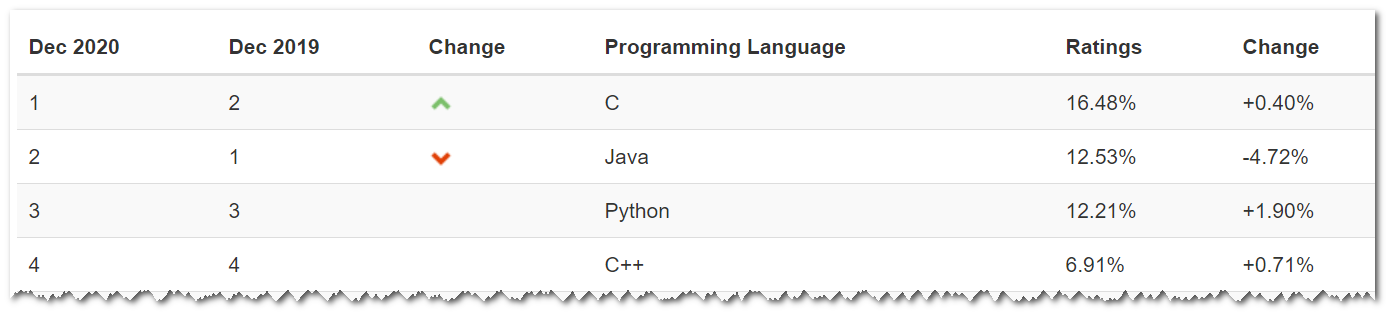
\includegraphics[width=\textwidth]{img/TIOBE_rating.png}

%Такою популярністю мова \texttt{C} зобов'язана концепції IoT (\textit{Internet of Things}) -- концепції мережі передачі даних між фізичними об'єктами («речами»), які обладнані вбудованими засобами та технологіями для взаємодії один з одним або із зовнішнім середовищем. Мова \texttt{C} підходить якнайкраще для створення невеликих пристроїв, яким вкрай важлива продуктивність за умови доступності вкрай обмежених апаратних ресурсів як об'єм пам'яті, обчислювальна потужність процесора тощо. 


%Актуальність вивчення дисципліни «Мікропроцесорна техніка» обумовлена необхідністю подальшого застосування в професійній діяльності фахівцями відповідних кваліфікацій знань і умінь в області апаратної реалізації і програмування мікропроцесорних засобів, програмних та апаратних інтерфейсів.
%
%Метою викладання навчальної дисципліни є формування знань в області мікропроцесорної техніки, що дозволяють аналізувати і проектувати мікропроцесорні пристрої.
%
%Публікація висвітлює один з аспектів проблеми проектування мікропроцесорних систем «без прив'я\-зу\-ван\-ня» до конкретного сімейства мікропроцесорів. Поданий матеріал орієнтований на вузьке коло студентів, які мають лише загальне уявлення про основи електроніки та схемотехніки, а при викладенні матеріалу використовується гіпотетичний мікропроцесор та пристрої зберігання інформації, які мають типові характристики  пристроїв, що випускаються в теперешній час.

%Розрахунково-графічна робота виконується студентами самостійно під керівниц\-твом викладача і для успішного її виконання важливим є вивчення нав\-чаль\-ної та методичної літератури з дисципліни «Мікропроцесорна техніка».

%Пропоновані методичні вказівки містять необхідну інформацію, яка сприятиме самостійному та грамотному виконанню розрахунково-графіч\-ної роботи. У відповідних розділах подано зміст і методику виконання розрахунків, завдання, порядок виконання та вимоги до оформлення текстової та графічної частини. Використовуючи рекомендований методичний підхід, студент зможе провести всі етапи проектування запам'ятовуючого пристрою для мікропроцесорної системи від постановки задачі до створення технічної документації.

«Мікропроцесорна техніка» є нормативною дисципліною в системі підготовки бакалавра, яка забезпечує теоретичну та практичну підготовку студентів для розв’язування фахових інженерних задач, а також використання спеціалізованого програмного забезпечення в процесі вив\-чен\-ня інших дисциплін, виконання курсових та дипломних робіт. Вивчення основ мікропроцесорної техніки ґрунтується на теоретичних положеннях курсу комп'ютерної техніки, програмування та алгоритмізації.

Дисципліна належить до тих фундаментальних дисциплін, які розвивають у студентів практичні навички, що стануть в пригоді як в процесі навчання, так і в професійній діяльності молодого фахівця. Основна задача курсу -- дати студентам знання у сфері застосування сучасних інформаційних технологій, забезпечити фундаментальність освіти майбутніх фахівців, а також навчити самостійно обирати та використовувати сучасний комп’ютерний інструментарій для вирішення фахових завдань. Знання та практичний досвід, набуті в процесі вивчення дисципліни, дозволять розширити можливості студентів при засвоєнні інших спеціальних дисциплін. 

\textit{Метою} навчальної дисципліни «Мікропроцесорна техніка» є розвиток алгоритмічного мислення, вивчення теоретичних основ і практичних засад проектування програмного забезпечення з використанням мов програмування низького рівня; отримання практичних навичок створення мікропроцесорних систем; набуття навичок роботи зі спеціалізованим програмним забезпеченням, трансляції програм в машинні коди, компонування машинного коду в пам'яті мікропроцесорної системи.

\textit{Предметом} вивчення дисципліни є проектування алгоритмів вирішення обчислювальних задач; створення програм та отримання машинного коду, придатного до вконання конкретним мікророцесором; ство\-рен\-ня елементарної мікропроцесорної системи, здатної виконувати елементарні обчислювальні завдання, оформлені відповідним чином.

Розрахунково-графічна робота з дисципліни «Мікропроцесорна техніка» є невід’ємною частиною навчального процесу, в ході виконання якої студенти набувають не лише необхідних навичок самостійної роботи, а й безпосередньо беруть участь у вирішенні практичних технічних задач. Метою даних методичних вказівок є викладення основних вимог до виконання та оформлення розрахунково-графічної роботи.
%!TEX root = ../mtrgrmetod.tex
\chapter{Основні положення}
Розрахунково-графічна робота (РГР) з дис\-цип\-ліни «Мікропроцесорна техніка» є важливою складовою частиною підготовки технічних фахівців галузей знань 12 -- «Інформаційні технології» та 15 -- «Автоматизація та приладобудування». Написання розрахунково-графічної роботи є обов’язковим етапом у вивченні програмного матеріалу названої дисципліни.

\textit{Метою} виконання розрахунково-графічної роботи є поглиблення набутих теоретичних знань з дисципліни «Мікропроцесорна техніка»; формування практичних навичок алгоритмізації та програмування, вирішення актуальних питань, пов’язаних з проектуванням мікропроцесорних систем; застосування набутого студентами у процесі навчання науково-технічного потенціалу.

У процесі досягнення зазначеної мети вирішуються такі \textit{завдання}:
\begin{itemize}
\item закріпити та поглибити знання з дисципліни «Мікропроцесорна техніка»;
\item систематизувати методичний інструментарій, оволодіти кон\-крет\-ни\-ми комп'ютерними засобами проектування;
\item сформулювати задачу на проектування та обґрунтувати методи й підходи до подальшої формалізації;
\item логічно і послідовно пройти всі етапи розрахунку та розробки;
\item проаналізувати результати, зробити відповідні вис\-нов\-ки.
\end{itemize}

\textit{Мета} і \textit{завдання} в межах виконання РГР визначаються її темою, структурою, специфікою об’єкта, предмета та інформаційною базою для проведення розрахунків.

Виконання студентами розрахунково-графічної роботи сприяє поєднанню в цілісну систему знань із галузі проектування мікропроцесорних засобів, що, в свою чергу, дозволяє їм –- майбутнім інженерам -- сформувати чіткі уявлення про функціонування таких пристроїв та навчитись використовувати їх на практиці.

%Керівник розрахунково-графічної роботи надає допомогу в уточненні змісту, скла\-дан\-ні завдання для виконання курсової роботи. Керівник також сприяє процесу збирання та отримання необхідного матеріалу для написання курсової роботи, рекомендує основну та додаткову літературу, проводить регулярні консультації; розробляє календарний графік виконання етапів роботи та слідкує за його дотриманням, перевіряє роботу, робить відповідні зауваження і вирішує питання про можливість допуску до захисту.

На початку семестру студент отримує індивідуальне завдання на розрахунково-графічну роботу, оформлене відповідно до вимог, що висуваються до такого роду документів. Як правило, індивідуальне завдання -- це аркуш паперу формату А4, на якому в стислій формі подаються вихідні дані для проведення роботи, визначаються числові значення необхідних параметрів та наводиться орієнтовний зміст роботи. Пакет індивідуальних завдань для студентів розглядається на засіданні кафедри і візується завідувачем кафедри на початку семестру. При отриманні індивідуального завдання у відповідній графі бланка студент ставить свій підпис. Свій підпис у відповідній графі ставить і керівник розрахунково-графічної роботи. Варіанти завдань наведені в додатку \ref{apdx:tasks} даних методичних вказівок.

Після отримання індивідуального завдання студент розробляє план роботи, який узгоджує з керівником. На базі розробленого плану формується зміст роботи та перелік необхідних розділів та додатків пояснювальної записки.

Після того, як буде сформовано зміст роботи, студент приступає безпосередньо до виконання робіт, окреслених розробленим планом, та формування пояснювальної записки згідно з сформованим змістом.

Виконання розрахунково-графічної роботи передбачає вивчення літературних джерел і підбір ілюстративного матеріалу. В першу чергу доцільно звертатися до навчальних посібників, які в системному порядку викладають основний зміст курсу. Інформаційною базою для виконання розрахунково-графічної роботи є технічна література у галузі; підручники і навчальні посібники, які в системному порядку викладають основні проблемні та актуальні питання цифрової й мікропроцесорної техніки.

%Особливу увагу слід приділити вивченню змісту основоположних теоретичних і практичних питань моделювання і організації та проведення обчислювального експерименту. При вивченні монографій, журнальних статей, іншої спеціальної літератури з питань, що безпосередньо відносяться до теми курсової роботи, необхідно скласти конспект, викладаючи зміст своїми словами. Такий підхід дозволить забезпечити правильне розуміння вивченого матеріалу, а також дасть можливість самостійно викласти зміст курсової роботи. В якості ілюстративного матеріалу слід підібрати заповнені аналітичні таблиці, графіки, схеми, алгоритми рішення завдань, малюнки, схеми взаємозв'язку показників, і інше.
%!TEX root = ../mtrgrmetod.tex
\chapter{Вимоги до оформлення}

Пояснювальна записка до розрахунково-графічної роботи ви\-ко\-ну\-єть\-ся за ДСТУ 3008-2015. Мова розрахунково-графічної роботи державна, стиль науковий, чіткий, без орфографічних і синтаксичних помилок; послідовність ло\-гіч\-на.

%\vspace{8mm}

\section{Вимоги до оформлення текстової частини}

Текст розрахунково-графічної роботи друкується на комп’ютері з одного боку стандартного аркуша паперу формату A4 ($210\!
\times\!297$ мм). Гарнітура Times New Roman, розмір шрифту 14 пунктів, інтервал 1,5 ($\approx$~28-30 рядків на сторінку). При написанні дотримуються таких розмірів полів: верхній, лівий і нижній -- не менше 20 мм, правий -- не менше 10 мм. Абзаци в тексті починають відступом, що дорівнює 1,27~см.

Під час виконання РГР потрібно дотримуватись рівномірної щільності, контрастності й чіткості зображення. Всі лінії, літери, цифри і знаки мають бути чіткими та однаково чорними впродовж усієї роботи.

Номери сторінок потрібно проставляти арабськими цифрами у правому верхньому кутку аркуша без крапки в кінці, дотримуючись наскрізної нумерації впродовж усього тексту роботи. Титульний аркуш вносять до загальної нумерації сторінок роботи, проте номер сторінки на титульному аркуші не проставляють.

Заголовки структурних частин (розділів) розрахунково-графічної роботи пишуть великими літерами симетрично до тексту, крапка в кінці заголовка не ставиться. Переноси частини слів в заголовку не допускаються, на інший рядок слово переноситься повністю. Якщо заголовок складається з двох речень, то вони розділяються крапкою. Кожний наступний розділ роботи починають з нової сторінки. Розділи нумеруються арабськими цифрами в межах всієї розрахунково-графічної роботи, проте розділам «ЗМІСТ», «ВСТУП», «ВИСНОВКИ», «ПЕРЕЛІК ПОСИЛАНЬ» номера не присвоюють. Крапка після цифри не проставляєься. Заголовки розділів відділяють знизу від основного тексту порожнім рядком або інтервалом в 1--1,5 розміру основного шрифту.

Заголовки підрозділів пишуться малими літерами окрім першої великої і розміщуються з абзацу. Переноси частини слів в підзаголовку не до\-пус\-ка\-ють\-ся, на інший рядок слово переноситься повністю. Якщо підзаголовок складається з двох речень, то вони розділяються крапкою. Не допускається розміщувати назву підрозділу, а також пункту й підпункту в нижній частині сторінки, якщо після неї розміщено тільки один рядок тексту. Підрозділи нумерують арабськими цифрами в межах розділу («1.1 Перший підрозділ першого розділу», «2.3 Третій підрозділ другого розділу»), крапку після останньої цифри не проставляють. Заголовки підрозділів відділяють знизу і згори від основного тексту порожнім рядком або інтервалом в 1--1,5 розміру основного шрифту.

Формули, що входять до розрахунково-графічної роботи, нумерують в межах розділу. Номер формули складається з номера розділу та порядкового номера формули, розділених крапкою. Номер формули розташовують з правого боку на рівні формули в круглих дужках. По\-си\-лан\-ня в тексті на номер формули дають в дужках, наприклад, «... за формулою (\ref{eq:explan})». За необхідності вказують одиницю вимірювання, беручи її в квадратні дужки

\begin{equation}
\label{eq:explan}
I = \frac{U}{R}~[A].
\end{equation}

Числову підстановку і розрахунок виконують з нового рядка не нумеруючи. Одиницю вимірювання беруть в круглі дужки. Наприклад,

$$I = \frac{220}{100}~(\text{А}).$$

Розмірність одного й того ж параметра в межах документа має бути однаковою. Якщо формула велика, то її можна переносити в на\-ступ\-ні рядки. Перенесення виконують тільки математичними знаками, повторюючи знак на початку наступного рядка. При цьому знак мно\-жен\-ня «$\cdot$» замінюють знаком «$\times$».

Пояснення символів та числових коефіцієнтів наводять під формулою. Пояснення кожного символа подається з нового рядка в тій послідовності, в якій символи зустрічаються в формулі. Перший рядок пояснення починається зі слова «де» без двокрапки після нього.

\begin{equation}
T = 2\pi\sqrt{\frac{m}{k}}, 
\end{equation}

\textit{
\begin{explanation}
\fitem $k$ -- коефіцієнт жорсткості пружини; 
\item $m$ -- маса тягарця.
\end{explanation}}

Формула є частиною речення, тому до неї застосовують такі ж правила граматики, як і до інших членів речення. Якщо формула зна\-хо\-дить\-ся в кінці речення, то після неї ставлять крапку. 

Формули, що записані одна за одною та не розділені текстом, розділяються комою. Рівняння і формули потрібно виділяти з тексту в окремий рядок. Формули відділяють знизу і згори від основного тексту порожнім рядком або інтервалом в 1--1,5 розміру основного шрифту.

Ілюстративні матеріали (таблиці і рисунки) розміщуються в тексті пояснювальної записки до розрахунково-графічної роботи або ви\-но\-сять\-ся в додатки. Ілюстрація має розташовуватись одразу після посилання на неї в тексті, або на наступній сторінці, якщо для розміщення її на поточній сторінці не вистачає місця.

Всі ілюстрації нумеруються арабськими цифрами в межах розділу і мають мати назву. Номер ілюстрації складається з номера розділу та порядкового номера ілюстрації, розділених крапкою, а назва ілюстрації подається після номера і відділяється від нього знаком «тире», на\-прик\-лад, «Рисунок 1.1 -- Схематичне зображення процесу переробки», «Таблиця 1.1 -- Результати комп'ютерного моделювання». Крапка в кінці заголовка ілюстрації не ставиться.

Рисунки підписують знизу симетрично до тексту і відділяють від основного тексту порожнім рядком або інтервалом в 1--1,5 розміру основного шрифту.

Таблиці підписують згори вирівнюючи назву по лівому краю таблиці і відділяють від основного тексту порожнім рядком або інтервалом в 1--1,5 розміру основного шрифту.

У разі перенесення частини таблиці на інший аркуш (сторінку) слово «Таблиця» та її номер вказують лише один раз -- ліворуч над першою частиною таблиці; над іншими частинами пишуть «Продовження табл.» із зазначенням номера таблиці, наприклад: «Продовження табл. 1.2».

Ілюстративний матеріал може бути оформлений у вигляді додатків. Додатки являють собою окремі розділи пояснювальної записки до розрахунково-графічної роботи, що розташовуються після переліку посилань. Як і будь-який розділ додатки мають відображатись в змісті пояснювальної записки і мати наскрізну нумерацію сторінок.

На відміну від звичайних розділів заголовок додатка записують маленькими літерами окрім першої великої і позначають великими літерами української абетки, починаючи з А, за винятком літер Ґ, Є, З, І, Ї, Й, О, Ч, Ь, наприклад, «Додаток А».  Заголовок додатка розташовують симетрично відносно тексту окремим рядком. Кожний наступний додаток починають з нової сторінки.

Текст кожного додатка, за необхідності, може бути поділений на розділи та підрозділи, пронумеровані в межах кожного додатка: перед кожним номером ставлять позначення додатка (літеру) і крапку, нап\-рик\-лад: «А.2» (другий розділ додатка А). Рисунки, таблиці та формули, розміщені в додатках, нумерують у межах кожного додатка, наприклад: «Рисунок Д.1.2» (другий рисунок першого розділу додатка Д).

При оформленні списку використаної літератури бібліографічний опис складають безпосередньо за друкованим текстом або виписують з каталогів і бібліографічних покажчиків повністю без пропусків будь-яких елементів, скорочення назв і т. ін.

Список використаних джерел має мати суцільну нумерацію. Використані джерела можна розміщувати в один з таких способів: за абет\-кою (за першою літерою прізвища автора або першого слова заголовка), у порядку розташування посилань у тексті. Оформлення літературних джерел здійснюється відповідно до вимог нормативних документів рекомендованих кафедрою.

Оформлена відповідно до сформульованих вимог та повністю укомплектована розрахунково-графічна робота має бути переплетена (зброшурована).

На першій (титульній) сторінці студент має поставити свій підпис та дату остаточного завершення роботи. Зразок оформлення титульного аркуша наведений в додатку \ref{apdx:title}.

%\newpage

\section{Вимоги до оформлення графічної частини}

Загальні вимоги і правила виконання схем встановлює ГОСТ 2.702-84 ЄСКД. Принципова схема є найповнішою електричною схемою виробу, на якій зображають всі електричні елементи і пристрої, потрібні для здійснення та контролю електричних процесів, всі електричні зв’язки між ними, а також електричні елементи, якими закінчуються вхідні і вихідні ланцюги.

До складу принципової схеми входять:
\begin{enumerate}
\item умовні графічні позначення електричних елементів і електричні зв’язки між ними;
\item позиційні літерно-цифрові позначення електричних елементів;
\item написи, що характеризують вхідні і вихідні ланцюги;
\item перелік елементів.
\end{enumerate} 

Принципові схеми мають бути максимально наочними, зручними для читання і найкращим чином відображати логіку розвитку процесу у виробах. Все це досягається дотриманням таких умов:

\begin{itemize}
\item елементи, що спільно виконують деякі функції (функціональні групи), потрібно на схемах групувати поблизу один від одного;
\item елементи всередині функціональних груп потрібно розташовувати так, щоб конфігурація ланцюгів була простою (кількість зламів і перетинів ліній має бути мінімальною);
\item функціональні групи елементів потрібно розташовувати на схемі в послідовності, відповідній розвитку процесу зліва направо;
\item всі додаткові і допоміжні функціональні ланцюги (елементи і зв’язки між ними) потрібно виводити зі смуги, зайнятої основними ланцюгами.
\end{itemize}

Схеми виконуються згідно з ГОСТ 2.702-84 без дотримання масштабу, дійсне просторове розташування елементів або не враховується взагалі, або враховується приблизно. Електричні елементи зображуються умовними графічними позначеннями (УГП).

Лінії електричного зв’язку на принциповій схемі носять умовний характер і не є зображенням реальних дротів. Лінії зв’язку між елементами схеми розташовують тільки горизонтально або вертикально, вони мають мати найменшу кількість зламів і взаємних перетинів.

Нормативний документ встановлює товщину ліній зв’язку від 0,2 до 1 мм залежно від формату схеми і розмірів графічних позначень. Товщина, що рекомендується -- від 0,3 до 0,4 мм.

Товщина лінії зв’язку дорівнює товщині ліній УГП. Відстань між двома паралельними лініями зв’язку — не менше 3 мм, а між окремими графічними зображеннями — не менше 2 мм.
На вільному полі схеми поміщають діаграми, таблиці, текстові вказівки.

Для компактності схеми, а також при великій насиченості схеми умовними графічними позначеннями, допускається всі позначення пропорційно зменшувати: при цьому проміжок між двома сусідніми лініями УГП має бути не менше 1,0 мм. З метою більшої наочності зображення на принциповій електричній схемі дозволяється переміщення елементів схеми на полі креслення без порушення принципів побудови самої схеми.

Для спрощення схеми допускається декілька електрично не пов’я\-за\-них ліній зв’язку зливати в лінію групового зв’язку (шину), як показано на рисунку~\ref{fig:shina}. Від задіяних контактів елемента {\gostfnt DD1}, що ліворуч, йдуть лінії зв’яз\-ку, які мають власну нумерацію і злиті умовно в одну лінію (шину), яка має більш товсте накреслення. У міру потреби від
цієї лінії відводять дроти (1, 2, 3, 4), підключені до елементів {\gostfnt DD2-DD5}.

\begin{figure}[h]
%\noindent
\centering
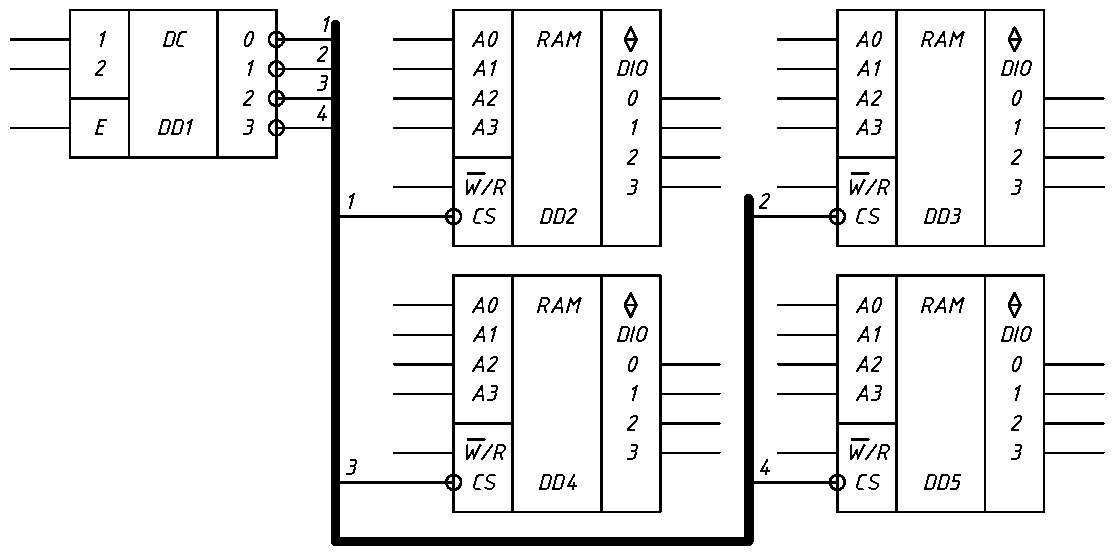
\includegraphics[width=\textwidth]{img/shina-crop.pdf}
\caption{Оформлення лінії групового зв'язку (шини)}
\label{fig:shina}
\end{figure}

Для однозначного визначення елементів, що входять до складу виробу і зображених на схемі, кожному елементу або пристрою схеми присвоюють літерно-цифрове позиційне позначення згідно з ГОСТ 2.710-81.

	Позиційне позначення в загальному випадку складається з трьох частин. У першій частині вказують вид елемента (пристрою) однією або декількома літерами, наприклад, {\gostfnt R} — резистор, {\gostfnt С} — конденсатор (для уточнення виду елемента допускається застосовувати двох літерний код, наприклад, для цифрової мікросхеми — {\gostfnt DD}); у другій частині — порядковий номер елемента або пристрою в межах даного виду, наприклад: {\gostfnt R1, R2, ..., R6}\textit{;} {\gostfnt С1, С2, ..., С5}\textit{;} {\gostfnt DD1, DD2}\textit{;} у третій частині допускається вказувати відповідне функціональне призначення, наприклад {\gostfnt C2I} -- конденсатор {\gostfnt С2}, що використовується як інтегрувальний. 

Позиційні позначення елементам (пристроям) присвоюють починаючи з одиниці в межах групи елементів (пристроїв) з однаковими позиційними позначеннями, за послідовністю розташування елементів на схемі, рахуючись згори вниз, зліва направо. Цифри порядкових номерів і їх літерні позиційні позначення виконують одним розміром шрифту.

Дані про елементи, що входять до складу виробу і зображені на схемі, записують в перелік елементів, який поміщають на першому аркуші схеми або виконують у вигляді самостійного документа певного формату (рис. \ref{fig:perelik}). 

\begin{figure}[h]
%\noindent
\centering
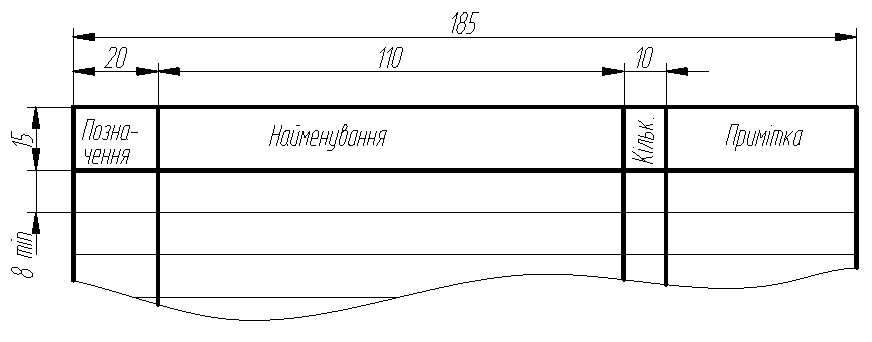
\includegraphics[width=\textwidth]{img/perelik-crop.pdf}
\caption{Оформлення переліку елементів}
\label{fig:perelik}
\end{figure}

У першому випадку перелік оформляється у вигляді таблиці, що заповнюється зверху вниз. Її розташовують, як правило, над основним написом на відстані не менше 12 мм від неї. Продовження переліку поміщають зліва від основного напису, повторюючи головку таблиці. У другому випадку перелік елементів виконується на
форматі А4 з основним написом згідно з ГОСТ 2.104–68 (форма 2 і 2а), з присвоєнням шифру, що складається з літери П (перелік) і коду схеми, до якої випускається перелік, наприклад: ПЕ3 — (П) перелік елементів до (Е) електричної (3) принципової схеми. У графах переліку елементів указують такі дані:

\begin{itemize}
\item у стовпці «Поз. позначення» наводяться позиційні позначення елементів (пристроїв);
\item у стовпці «Найменування» — найменування елементів (пристроїв) відповідно до документа, на підставі якого цей елемент (пристрій) застосований, а також позначення цього документа (основний конструкторський документ: ГОСТ, ТУ);
\item у стовпці «Кількість» — кількість однакових елементів;
\item у стовпці «Примітка» — технічні дані елемента, що не містяться в його найменуванні (за необхідності).
\end{itemize}

Допускається всі відомості про елементи поміщати поряд з їх зображенням на вільному полі схеми. Зв’язок переліку елементів має здійснюватися через позиційні позначення.

Перелік заповнюється згори вниз як у випадку, коли перелік розташований на першому аркуші схеми, так і у разі виконання його у вигляді самостійного документа (рис. \ref{fig:elist}). Заповнення переліку проводять групами в алфавітному порядку літерно-цифрових позиційних позначень. Якщо на схемі застосовуються позиційні позначення з літер латинського і українського алфавітів, то в перелік спочатку записують елементи з позиційними позначеннями з літер латинського алфавіту, а потім -- українського. В межах кожної групи, що має однакові літерні позиційні позначення, елементи розташовуються за збільшенням порядкових номерів. Між окремими групами елементів рекомендується залишати декілька незаповнених рядків для внесення змін.

\begin{figure}[h]
%\noindent
\centering
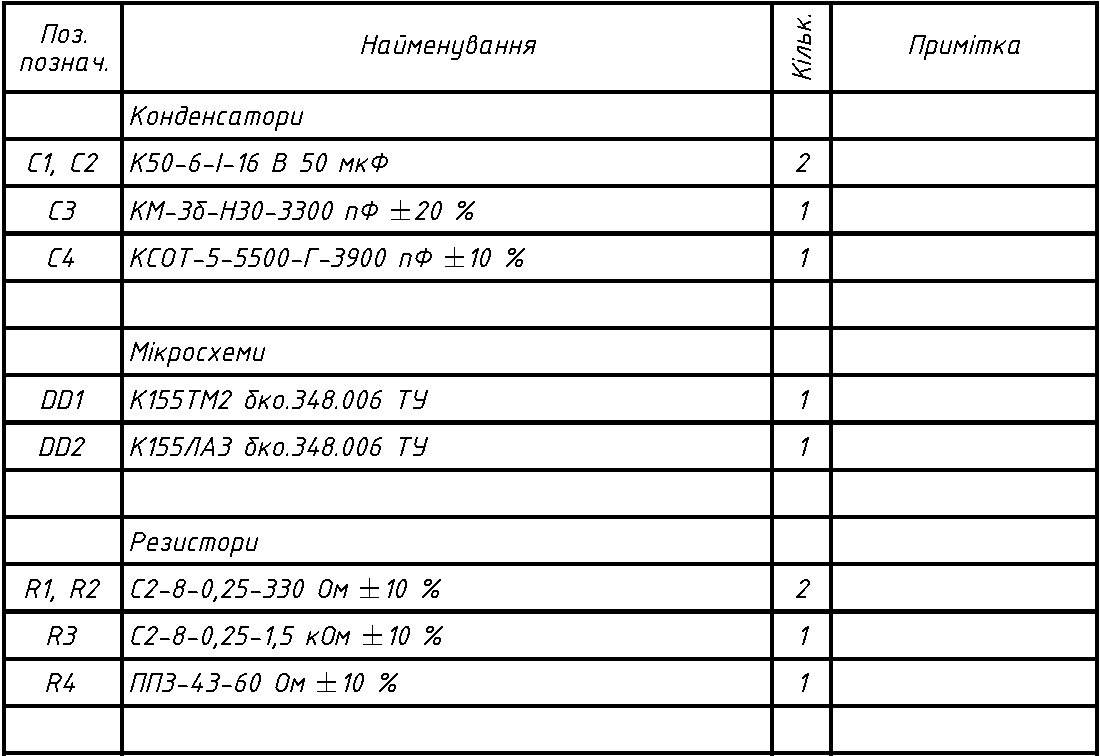
\includegraphics[width=0.9\textwidth]{img/elist-example.pdf}
\caption{Приклад заповнення переліку елементів}
\label{fig:elist}
\end{figure}
 
%!TEX root = ../mtrgrmetod.tex
\chapter{Розрахунок модуля оперативного запам'ятовувального пристрою}

%При матричной организации ИМС памяти (рис. 5.6) реализуется координатный принцип адресации ячеек. Адрес ячейки, поступающий по шине адреса ВМ, пропускается через логику выбора, где он разделяется на две составляющие: адрес строки и адрес столбца. Адреса строки и столбца запоминаются соответственно в регистре адреса строки и регистре адреса столбца микросхемы. Регистры соединены каждый со своим дешифратором. Выходы дешифраторов образуют систему горизонтальных и вертикальных линий, к которым подсоединены запоминающие матрицы, при этом каждый ЗЭ расположен на пересечении одной горизонтальной и одной вертикальной линии. 

%\section{ttt}

Незалежно від того, яким чином організована мікропроцесорна система, в її складі в будь-якому випадку має бути запам'ятовувальний пристрій. Як правило, в складі такої системи можна побачити постійний запам'я\-то\-ву\-валь\-ний пристрій та оперативний запам'ятовувальний пристрій, які поділять між собою адресний простір мікропроцесора, але, в окремих випадках номенклатура пристроїв зберігання інформації в складі мікропроцесорної системи буде ширшою.

%\vspace{8mm}

\section{Класифікація запам'ятовувальних пристроїв}

Класифікувати запам'ятовувальні пристрої (ЗП), які використовуються в мікропроцесорних системах сьогодні, можна за такими ознаками:
\begin{enumerate}
 \item \textbf{за місцем} розташування відносно обчислювального прис\-трою:
   \begin{enumerate}
   \item зовнішні ЗП,
   \item внутрішні ЗП;
   \end{enumerate}
 \item \textbf{за призначенням}:
   \begin{enumerate}
   \item надоперативні ЗП (НОЗП) -- мають швидкодію, сумірну зі швидкодією обчислювального пристрою. Використо\-ву\-ють\-ся для зберігання результатів проміжних операцій. У мікропроцесорах роль НОЗП виконує регістрова пам'ять -- вбудовані в мікропроцесор регістри загального призначення;
   \item оперативні ЗП (ОЗП) -- енергозалежні ЗП, вико\-рис\-то\-ву\-ють\-ся для первинного зберігання інформації, що вво\-дить\-ся. При відсутності живлення інформація втрачається;
   \item постійні ЗП (ПЗП) -- енергонезалежні ЗП, ви\-ко\-рис\-то\-ву\-ють\-ся для зберігання інформації і за відсутності напруги живлення;
   \item буферні ЗП (БЗП) -- призначені для проміжного зберігання інформації при її обміні між пристроями, що працюють з різною швидкістю. Цю роль виконують регістрові схеми або ОЗП малого обсягу;
   \item зовнішні ЗП (ЗЗП) використовуються для зберігання великого обсягу інформації на зовнішньому, щодо обчислювального пристрою, носії, як правило, магнітному;
   \end{enumerate}\newpage
 \item \textbf{за фізичним принципом} дії:
   \begin{enumerate}
   \item магнітні,
   \item напівпровідникові,
   \item оптичні;
   \end{enumerate}
 \item \textbf{за способом зберігання} інформації:
   \begin{enumerate}
   \item статичні,
   \item динамічні;
   \end{enumerate}
 \item \textbf{за способом доступу} до комірок:
   \begin{enumerate}
   \item адресні ЗП -- код на адресному вході вказує на комірку, з якою ведеться обмін даними;
   \item послідовні ЗП -- звернення до комірки з заданою адресою передбачає виконання попередніх звернень до всіх комірок, які мають молодші адреси;
   \item асоціативні ЗП -- пошук інформації відбувається за деякою ознакою, а не за її розташуванням в пам'яті.
   \end{enumerate}        
\end{enumerate}

\vspace{0.1cm}

Для позначення запам'ятовувальних пристроїв ОЗП та ПЗП з одної класифікаційної категорії «за призначенням» в літературі використовують сталі англомовні скорочення RAM та ROM. Однак ці абревіатури характеризують пристрої з різних сторін. Так, RAM (\textit{англ. Random Access Memory -- пам'ять з довільним доступом}) вказує на те, що для доступу до певної комірки не потрібно попередньо звертатись до комірок з молодшими адресами. Сама ж пам'ять при цьому може бути енергозалежною або енергонезалежною. Так само ROM (\textit{англ. Read Only Memory -- пам'ять тільки для читання}) свідчить про те, що в такий пристрій записувати не можна. Але енергонезалежність пристрою передбачає і можливість запису. Не зважаючи на таку неточність ці абревіатури залишаються сталими та широковживаними у сфері комп'ютерної техніки для позначення ОЗП та ПЗП.

В свою чергу оперативні запам'ятовувальні пристрої RAM по\-ді\-ля\-ють\-ся на статичні -- SRAM (\textit{англ. Static RAM}) та динамічні -- DRAM (\textit{англ. Dynamic RAM}).

У статичних ОЗП запам'ятовувальними елементами є тригери, на відміну від динамічних ОЗП, в яких дані зберігають у вигляді зарядів конденсаторів, що утворюються елементами МОН-структур. Особливістю динамічних ОЗП є те, що запам'ятовувальні конденсатори з часом розряджаються, тому періодично дані мають регенеруватися.

Щільність пакування динамічних елементів пам'яті в кілька разів вища, ніж статичних, тому динамічні ОЗП характеризуються найбільшою інформаційною ємністю і невисокою вартістю, але мають більше енергоспоживання і меншу швидкодію.

\newpage

Постійна пам'ять типу ROM має такі різновиди:
\begin{enumerate}
\item інтегральні схеми, які програмуються при виготовленні з допомогою масок -- ``маскові'' ПЗП або ROM(M);
\item пам'ять, що програмується користувачем, -- ППЗП (програмовані ПЗП):
  {\begin{itemize}
  \item PROM -- дані в пам'ять записуються один раз,
  \item EPROM та EEPROM -- вміст пам'яті може бути змінений шляхом видалення інформації та запису нової.  
  \end{itemize}}
\end{enumerate}

В EPROM видалення інформації відбувається шляхом опромінення кристала ультрафіолетовими променями (ППЗП-УФ -- ПЗП з можливістю перепрограмування шляхом видалення інформації УФ опроміненням). В EEPROM видалення інформації відбувається електричними сигналами (ППЗП-ЕС -- ПЗП з можливістю перепрограмування з використанням електричних сигналів). Запис даних в обох випадках (EPROM та EEPROM) відбувається з використанням електричних сигналів.

%----------------------------------------------------------------
\section{Способи збільшення інформаційного обсягу ЗП}

При проектуванні модуля ЗП на заданих великих інтегральних схемах  (ВІС) часто доводиться вирішувати задачу збільшення загальної інформаційної ємності пам'яті мікропроцесорної системи. Як правило, ця задача вирішується трьома способами: 

\begin{enumerate}
 \item{збільшенням розрядності даних (розрядності слів),}
 \item{збільшенням кількості слів, що адресуються (збільшення роз\-ряд\-нос\-ті шини адреси),}
 \item{комбінований.}
\end{enumerate}

\begin{center}
\textit{Збільшення розрядності даних}
\end{center}

Збільшення розрядності даних досягається шляхом паралельного з'єднання адресних ліній декількох мікросхем ЗП. В такому випадку на всі мікросхеми ЗП одночасно подається однакова адреса. Входи $\overline{CS}$ та \textit{$\overline{W}\!\!$/$R$} з'єднуються між собою також паралельно, що забезпечує подачу сигналів керування на всі мікросхеми одночасно. Таким чином в довільний момент часу для обміну даними доступні всі мікросхеми ЗП.

В наведеному прикладі (рис.~\ref{fig:sch1}) ємність одної інтегральної схеми буде визначатись як 

$$M1 = 2^{10}\cdot1 = 1024~\text{(біти)},$$

\noindent
а ємність всієї структури

$$M = M1\cdot8 = 2^{10}\cdot1\cdot8 = 8192~\text{(біти)} = 1~\text{(Кбайт)}.$$

\begin{figure}[h]
%\noindent
\centering
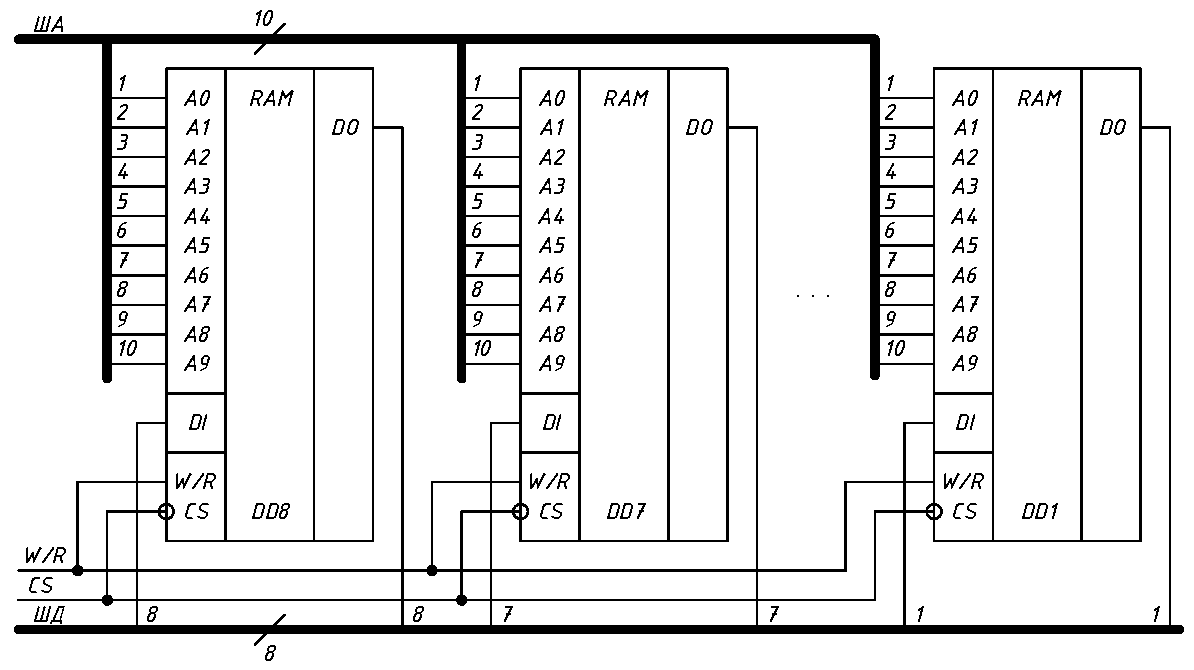
\includegraphics[width=\textwidth]{img/sch1-crop.pdf}
\caption{Збільшення розрядності даних}
\label{fig:sch1}
\end{figure}

Загальна інформаційна ємність в такому випадку змінюється за рахунок збільшення розрядності слів, що адресуються (з 1 біта для окремої ВІС до 1 байта для всього модуля ОЗП). Розрядність адреси ж всього модуля ОЗП залишається незмінною і збігається з розрядністю окремої ВІС, що дозволяє адресувати $2^{10} = 1024$ слова.  

\begin{center}
\textit{Збільшення кількості слів}
\end{center}

Для збільшення кількості слів, що адресуються, ви\-ко\-рис\-то\-ву\-єть\-ся дешифратор (\textit{англ. Decoder -- дешифратор}), на входи якого по\-да\-ють\-ся старші розряди шини адреси. Входи $\overline{CS}$ мікросхем ЗП під'єд\-ну\-ють\-ся до відповідних виходів дешифратора. Вхід $E$ дешифратора використовується як вхід дозволу роботи всієї схеми та використовується зовнішніми пристроями як вхід вибору кристала $\overline{CS}$. Проте в довільний момент часу для обміну даними доступна лише одна мікросхема ЗП в модулі. Входи \textit{$\overline{W}\!\!$/$R$} ЗП з'єднуються паралельно.

В наведеному прикладі (рис.~\ref{fig:sch2}) розрядність шини адреси збільшується з використанням дешифратора \textit{DD5}, на входи якого подаються старші розряди шини адреси. Входи $\overline{CS}$ окремих ВІС під'єднуються до відповідних виходів дешифратора. Вхід $E$ дешифратора використовується як вхід дозволу роботи всієї схеми та ідентифікується зовнішніми пристроями як вхід вибору кристала $\overline{CS}$. Входи \textit{$\overline{W}\!\!$/$R$} окремих ВІС з'єднуються між собою.

\begin{figure}[h]
%\noindent
\centering
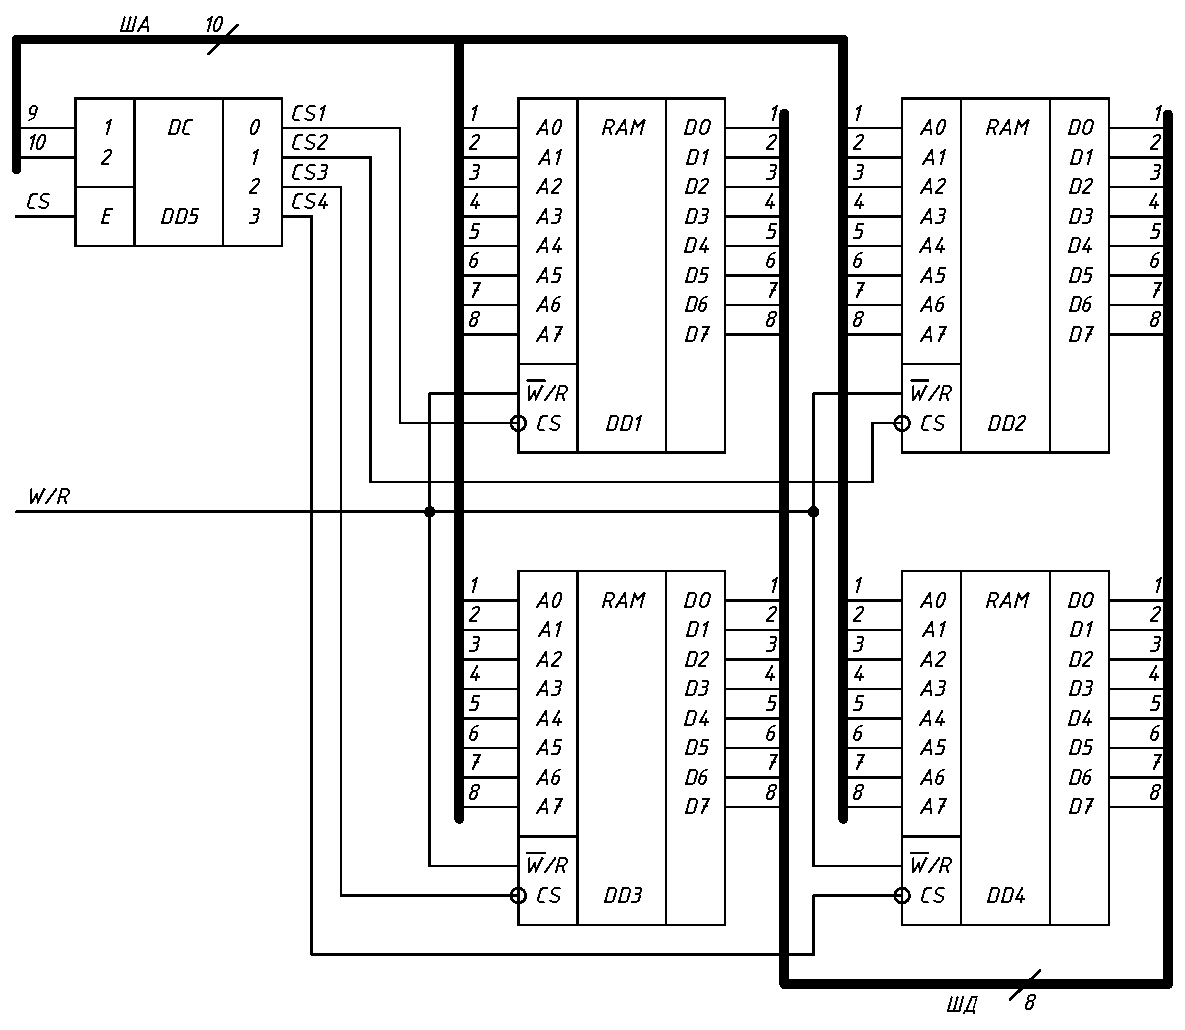
\includegraphics[width=\textwidth]{img/sch2(2)-crop.pdf}
\caption{Збільшення розрядності шини адреси}
\label{fig:sch2}
\end{figure}

Інформаційна ємність одної інтегральної схеми буде визначатись як

$$M1 = 2^{8}\cdot8 = 2048~\text{(бітів)},$$    

\noindent
а ємність всієї структури 

$$M = M1\cdot4 = 2^{8}\cdot8\cdot4 = 8192~\text{(біти)} = 1~\text{(Кбайт)}.$$

Загальна інформаційна ємність в такому випадку змінюється за рахунок збільшення кількості слів, що адресуються (з 256 для окремої ВІС до 1024 для всього модуля ОЗП). Розрядність слова залишається сталою як для модуля ОЗП в цілому, так і для окремої ВІС і складає 8~бітів. 

\begin{center}
\textit{Комбінований}
\end{center}

Комбінований спосіб передбачає і збільшення розрядності даних, і збільшення кількості слів, що адресуються. В такому випадку модуль ОЗП буде складатись із блоків, підключених за схемою збільшення розрядності шини адреси, а блоки збираються за схемою збільшення роз\-ряд\-нос\-ті даних.  

В наведеному прикладі (рис.~\ref{fig:sch3}) модуль ОЗП складається з чотирьох блоків організованих як $256\times8$, забезпечуючи загальну ємність запам'ятовувального пристрою 1024 байти або 1 Кбайт. В свою чергу кожен окремий блок складається з восьми ВІС, організованих як $256\times1$, здатних зберігати 256 бітів інформації.  

\begin{figure}[h]
%\noindent
\centering
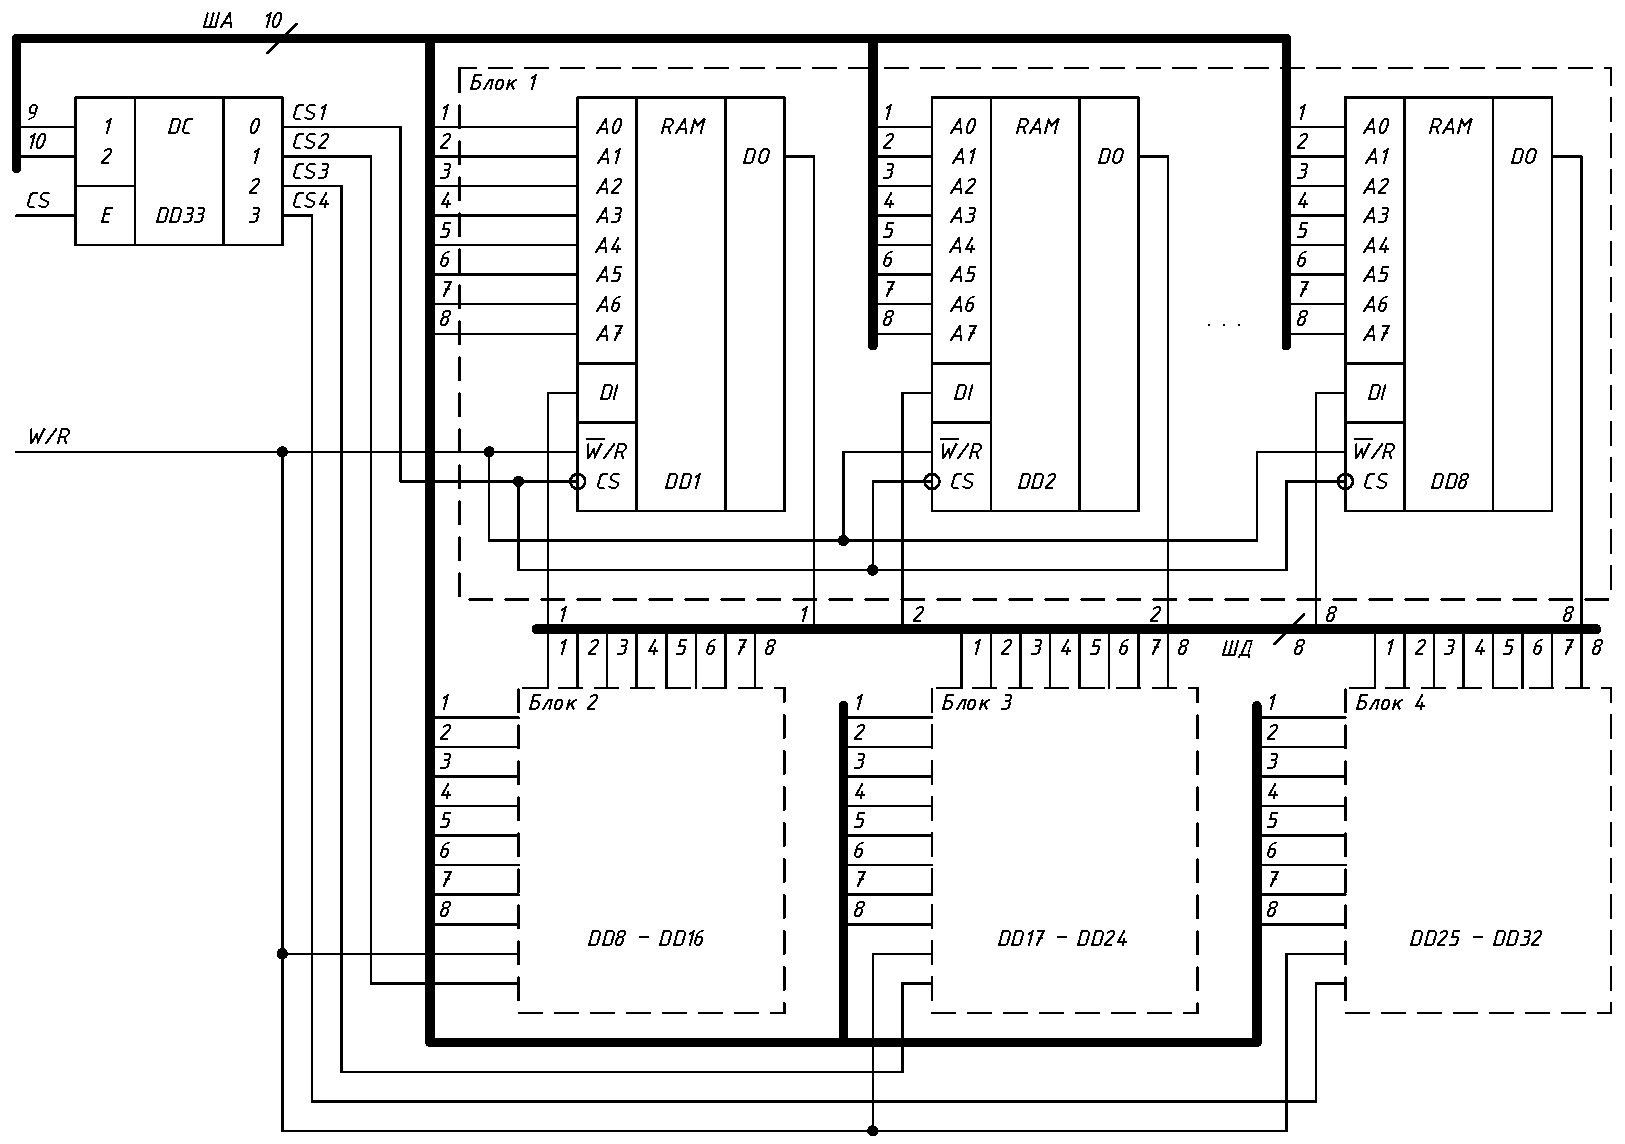
\includegraphics[width=0.99\textwidth]{img/sch3-crop.pdf}
\caption{Комбінований метод}
\label{fig:sch3}
\end{figure}

Інформаційна ємність одної інтегральної схеми буде визначатись як

$$M1 = 2^{8}\cdot1 = 256~\text{(бітів)}.$$    

В свою чергу інформаційна ємність блока буде визначатись як добуток інформаційної ємності одної ВІС на їх кількість в блоці

$$M_{\text{Б}} = 2^{8}\cdot1\cdot8 = 2048~\text{(біта)} = 256~\text{(байтів)},$$ 

\noindent
а інформаційна ємність всієї структури становитиме 

$$M = M_{\text{Б}}\cdot4 = 2048\cdot4 = 8192~\text{(біти)} = 1~\text{(Кбайт)}.$$

Загальна iнформацiйна ємнiсть в такому випадку змiнюється як за рахунок збiльшення розрядностi слiв, що адресуються (з 1 бiта для окремої ВIС до 1 байта для окремого блока), так і за рахунок збільшення кількості слів, що адресуються (з 256 слів для окремої ВІС або окремого блока до 1024 для всього модуля ОЗП). 

Наведені приклади наочно демонструють рiзнi підходи до вирішення задачі збільшення інформаційної ємності ЗП до 1 Кбайта. Очевидно, що в кожному окремому випадку саме заданий тип ВІС буде визначати спосіб проектування ОЗП.

\section{Розрахунок модуля ОЗП}

Базові розрахунки направлені на визначення кількості ВІС, потрібних для отримання шуканої інформаційної ємності всього модуля, та типу дешифратора для забезпечення коректного дешифрування адреси. Розглянемо на прикладі:

%---------------------------------------------------------------
%                         завдання
\par\bigskip 
\noindent\centerline{\begin{minipage}{0.95\textwidth}
\textit{розрахувати модуль ОЗП 64$\times$8 на основі мікросхем пам’яті 16$\times$4 із Z-станом. 	Накреслити схему електричну принципову модуля ОЗП для підключення до мікропроцесора. Для керування модулем використати лінії $\overline{CS}$ та          $\overline{W}\!\!$/$R$.}
\end{minipage}}\par\bigskip

1.~Визначаємо шукану інформаційну ємність модуля ОЗП в бітах

$$M = 64\cdot8 = 512~\text{(бітів)}.$$

2.~Визначаємо кількість мікросхем, що потрібні для реалізації необхідної розрядності даних (паралельне з'єднання ВІС). Розрядність заданої ВІС -- 4, розрядність даних, що вимагається завданням, -- 8, отже потрібно паралельно з'єднати дві мікросхеми.

Інформаційна ємність одної мікросхеми становитиме

$$M1 = 16\cdot4 = 64~\text{(біти)}.$$

Інформаційна ємність двох мікросхем, поєднаних в блок для розширення розрядності, становитиме

$$M_{\text{Б}} = M1\cdot2 = 16\cdot4\cdot2 = 128~\text{(бітів)}.$$

Розширення розрядності не забезпечує потрібної інформаційної ємності ОЗП, відповідно, доведеться використати комбінований спосіб збільшення обсягу ЗП.

\vspace{5mm}

3.~Визначаємо кількість блоків $k$, потрібних для реалізації шуканого обсягу $M$

$$k = \frac{M}{M_{\text{Б}}} = \frac{512}{128} = 4~\text{(блоки)}.$$

Блоки будемо підключати за схемою розширення розрядності шини адреси, тому потрібно буде використати дешифратор на чотири виходи (два входи).

Шина адреси модуля ОЗП шуканої інформаційної ємності шестирозрядна ($64 = 2^{6}$). Старші два розряди заводяться на входи дешифратора, молодші розряди, що залишились, заводяться паралельно на кожну окрему ВІС. Виходи дешифратора з'єднуються з входами вибору окремих блоків (\textit{CS1 -- CS4}), а лінія керування \textit{$\overline{W}\!\!$/$R$} підключається до відповідного входу кожної окремої ВІС в модулі (додаток \ref{apdx:ozpsch}).



%!TEX root = ../mtrgrmetod.tex
\nocite{*}

%ГОСТ 7.1 2003
%\bibliographystyle{ugost2003}

%ГОСТ 7.1 2003
\bibliographystyle{gost2003new}

%ДСТУ 3802:2015
%\bibliographystyle{gost2008new}
%\def\BibEmph#1{\emph{#1}}    %%% для краси
%\def\BibDash{} 

\bibliography{biblio_basic}
\appendix
%!TEX root = ../mtrgrmetod.tex
\chapter[(Обов'язковий) Завдання на РГР]{(Обов'язковий)\\ Завдання на РГР}\label{apdx:tasks}

Розрахувати модуль ОЗП на основі заданого типу мікросхем пам’яті із Z-станом. 	Накреслити схему електричну принципову модуля ОЗП для підключення до мікропроцесора. Для керування модулем використати лінії $\overline{CS}$ та \textit{$\overline{W}\!\!$/$R$}.

\renewcommand{\arraystretch}{1.2}

\begin{table}[h]
\leftskip=2.5em
\caption{Варіанти завдань}
\label{tab:tasks}
\begin{tabular}{|c|>{\raggedleft}m{1.6cm}@{\ $\times$\ }m{1.2cm} |>{\raggedleft}m{1.6cm}@{\ $\times$\ }m{1.0cm}|}
  \hline
  \multicolumn{1}{|c|}{№ варіанта}&\multicolumn{2}{c}{модуль ОЗП} & \multicolumn{2}{|c|}{тип ВІС} \\ 
  \hline\hline
  1  & 256  & 8  & 64   & 1 \\
  2  & 256  & 8  & 64   & 2 \\
  3  & 1024 & 8  & 64   & 4 \\
  4  & 128  & 16 & 64   & 8 \\
  5  & 256  & 8  & 128  & 1 \\
  6  & 512  & 8  & 128  & 2 \\ 
  7  & 1024 & 8  & 128  & 4 \\
  8  & 512  & 16 & 128  & 8 \\
  9  & 1024 & 8  & 256  & 1 \\
  10 & 1024 & 8  & 256  & 2 \\
  11 & 1024 & 8  & 256  & 4 \\
  12 & 4096 & 16 & 256  & 8 \\
  13 & 2048 & 8  & 512  & 1 \\
  14 & 1024 & 8  & 512  & 2 \\
  15 & 4096 & 8  & 512  & 4 \\
  16 & 2048 & 16 & 512  & 8 \\
  17 & 4096 & 8  & 1024 & 1 \\
  18 & 4096 & 8  & 1024 & 2 \\
  19 & 4096 & 8  & 1024 & 4 \\
  20 & 4096 & 16 & 1024 & 8 \\
  \hline
\end{tabular}
\end{table}

%!TEX root = ../mtrgrmetod.tex
\chapter[(Довідковий) Зразок оформлення титульного аркуша]{(Довідковий)\\ Зразок оформлення титульного аркуша}\label{apdx:title}

%\fbox{%
%\begin{minipage}[t][21cm][t]{\textwidth}
%\small{%
%\onespace
%%\begin{titlepage}
%  {\centering{Вінницький національний технічний університет}\\*Кафедра автоматизаціїї та інтелектуальних інформаційних технологій\\*}
%  \vfill
%  {\centering\Large{Розрахунково-графічна робота}\\}
%  \vspace{2em}
%  {\centering з дисципліни: <<Мікропроцесорна техніка>>\\на тему: {тема}\\}
%  \vfill
%  \hfill\begin{minipage}{0.54\textwidth}%0.6
%  Студента(ки)\hfill{II}\hfill курсу \hfill{1АКІТ-19б}\hfill групи\\
%  напряму підготовки: {напрям}\\
%  спеціальності: {спеціальність}, %\rightskip 0em plus 5em
%  \mbox{гкавтор}\\\\
%  Керівник: 
%  \hrulefill
%  Національна шкала \hrulefill \\\\
%  Кількість балів: \hrulefill~Оцінка: ECTS~\hrulefill\\~\\
%  \end{minipage}
%  \hangindent=3.5cm \hangafter=0 \par
%  \noindent
%  \begin{minipage}[t]{.342\textwidth}%.38
%   \begin{flushright}
%   Члени комісі:
%   \end{flushright}
%  \end{minipage}\hspace{.018\textwidth}%.02
%  \begin{minipage}[t]{.252\textwidth}%.28
%   \begin{center}
%    \hrulefill\\
%    \small(підпис)\\~\\
%    \hrulefill\\
%    \small(підпис)\\~\\
%    \hrulefill\\
%    \small(підпис)\\~\\
%   \end{center}
%  \end{minipage}\hspace{.036\textwidth}%.04
%  \begin{minipage}[t]{.252\textwidth}%.28
%   \begin{center}
%    \hrulefill\\
%    \small(прізвище та ініціали)\\~\\
%    \hrulefill\\
%    \small(прізвище та ініціали)\\~\\
%    \hrulefill\\
%    \small(прізвище та ініціали)\\~\\
%   \end{center}
%  \end{minipage}
%
%  \vfill
%  {\centering м.~Вінниця~--~{\the\year}~р.\\}
%  %\end{titlepage}
%  }
%\end{minipage}}

\setlength\parindent{0pt}
\begin{center}
\fbox{
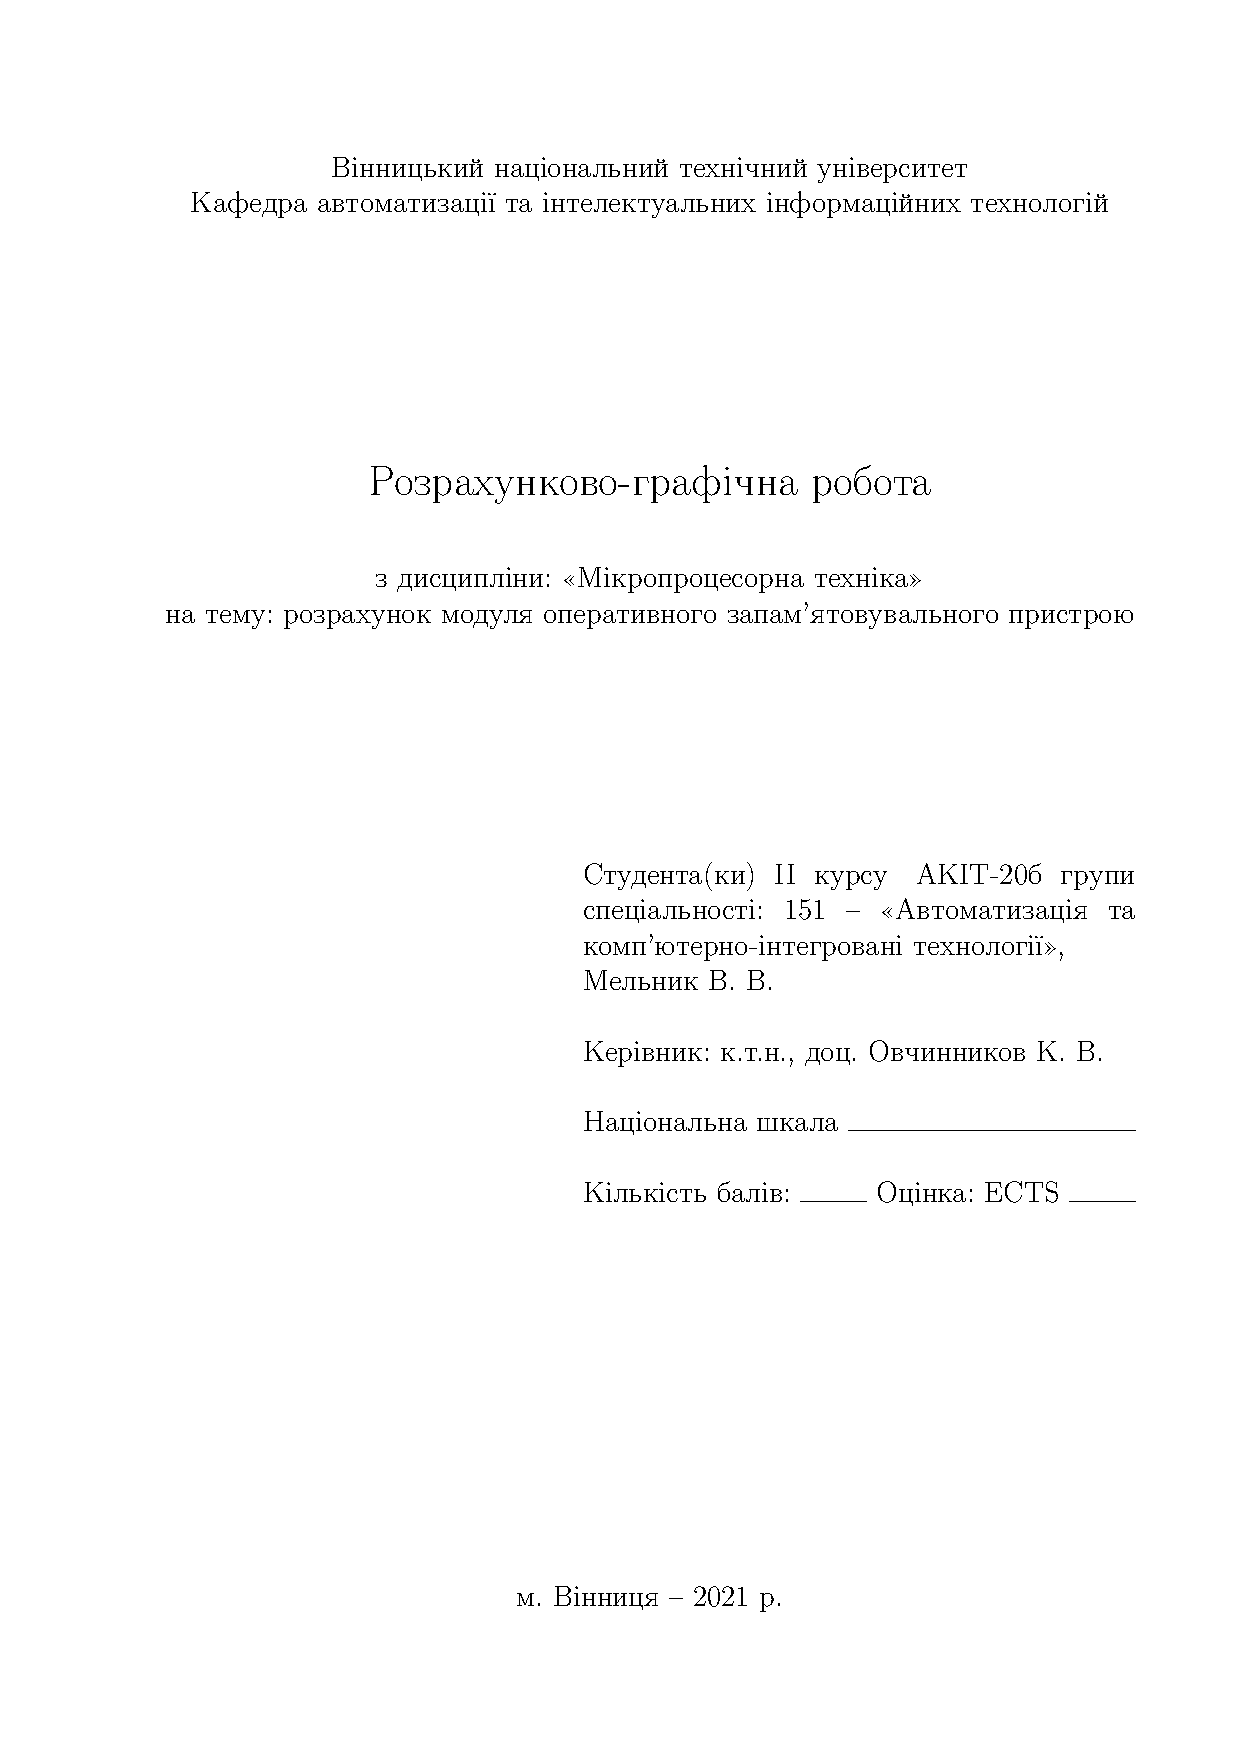
\includegraphics[width=0.7\pdfpagewidth,height=0.7\pdfpageheight]{img/rgrtitle.pdf}}
\end{center}
\newpage
%!TEX root = ../mtrgrmetod.tex

\acode{08-02}%
\bcode{РГР}%
\ccode{МТ}%
\dcode{13}%
\ecode{000}
\fcode{Е3}
\author{Мельник~В.~В.}%
\leader{Овчинников~К.}%
\reviewer{}%
\controller{}%
\approver{}%
\educationalabbr{ВНТУ}%
\group{АКІТ-20б}%
\title{Модуль ОЗП}%
\partdes{Схема електрична принципова}%

\begin{drawing}
%\appheadinhibit
\chapter[(Довідковий) Модуль ОЗП. Схема електрична принципова]{}
%Провести математичне моделювання процесу руху тіла в просторі для чого:
\begin{picture}(0,0)
\put(-70,-750){\hbox{\includegraphics{img/sch4.pdf}}}
\end{picture}
\label{apdx:ozpsch}
\end{drawing}

%\begin{drawing}
%\appheadinhibit
%\chapter[(Довідковий) Модуль ОЗП. Схема електрична принципова]{}
%%Провести математичне моделювання процесу руху тіла в просторі для чого:
%\includepdf[]{img/sch4.pdf}
%%\includepdf[picturecommand={\includegraphics[]{img/sch4.pdf}}]{img/sch4.pdf}
%\label{apdx:ozpsch}
%\end{drawing}

%\begin{elementlist}
%\category{category}
%\element{E1}{123}{4}{5}
%\element{E2}{123}{4}{5}
%\element{E1}{123}{4}{5}
%\element{E2}{123}{4}{5}
%\element{E1}{123}{4}{5}
%\element{E2}{123}{4}{5}
%\element{E1}{123}{4}{5}
%\element{E2}{123}{4}{5}
%\element{E1}{123}{4}{5}
%\element{E2}{123}{4}{5}
%\element{E1}{123}{4}{5}
%\element{E2}{123}{4}{5}
%\element{E1}{123}{4}{5}
%\element{E2}{123}{4}{5}
%\element{E1}{123}{4}{5}
%\element{E2}{123}{4}{5}
%\element{E1}{123}{4}{5}
%\element{E2}{123}{4}{5}
%\element{E1}{123}{4}{5}
%\element{E2}{123}{4}{5}
%\element{E1}{123}{4}{5}
%\element{E2}{123}{4}{5}
%\element{E1}{123}{4}{5}
%\element{E2}{123}{4}{5}
%\element{E1}{123}{4}{5}
%\element{E2}{123}{4}{5}
%\element{E1}{123}{4}{5}
%\element{E2}{123}{4}{5}
%\element{E1}{123}{4}{5}
%\element{E2}{123}{4}{5}
%\element{E1}{123}{4}{5}
%\element{E2}{123}{4}{5}
%\element{E1}{123}{4}{5}
%\element{E2}{123}{4}{5}
%\element{E1}{123}{4}{5}
%\element{E2}{123}{4}{5}
%\element{E1}{123}{4}{5}
%\element{E2}{123}{4}{5}
%\element{E1}{123}{4}{5}
%\element{E2}{123}{4}{5}
%\end{elementlist}

%!TEX root = ../mtrgrmetod.tex
\newpage
\thispagestyle{empty}
\onespace
\begin{center}
\textit{Електронне навчальне видання\\
комбінованого використання\\
Можна використовувати в локальному та мережному режимах}
\vfill
\large{\textbf{Методичні вказівки\\ до виконання розрахунково-графічної роботи з дисципліни «Мікропроцесорна техніка» для студентів усіх освітніх програм і форм навчання спеціальностей: 126 -- «Інформаційні системи та технології», 151 -- «Автоматизація та комп’ютерно-інтегровані технології»}}
\end{center}

%\vspace{0.8cm}
\begin{tabbing}
\noindent Укладачі: \= Костянтин Вячеславович Овчинников,\\
~ \> Володимир Володимирович Гармаш
\end{tabbing}

%\vspace{0.2cm}
\noindent Рукопис оформив К. Овчинников

\vspace{0.4cm}
\noindent Редактор В. Дружиніна

\vfill
\vfill

\begin{center}
\small{
Підписано до видання 15.04.2021 р.\\
Гарнітура \garnitura.\\
Зам. № P2021-008.\\
\vfill
\vfill
Видавець та виготовлювач\\
Вінницький національний технічний університет,\\
інформаційний редакційно-видавничий центр.\\
ВНТУ, ГНК, к. 114.\\
Хмельницьке шосе, 95,\\
м. Вінниця, 21021.\\
Тел. (0432) 65-18-06.\\
\textbf{press.vntu.edu.ua;}\\
\textit{Email:} irvc.vntu@gmail.com.\\
Свідоцтво суб’єкта видавничої справи\\
серія ДК № 3516 від 01.07.2009 р.}
\vfill
\vfill
\vfill

\end{center}

\end{document}